\chapter{Implementation}
\label{cap5}



\section{Graphical editor}\label{editor}

In order to create the Graphical Editor, described in section \ref{plutoGraphicalEditor}, we have chosen to exploit the GEF (Graphical Editing Framework) project. This framework is a Java technology and it is part of the Eclipse framework developed by IBM.
It gives developers a full solution for graphical modeling of a Java object model, and it can be used in conjunction with other technologies such as EMF (Eclipse Modeling Framework) or GMF (Graphical Modeling Framework), to enable the creation of a complete graphical modeling suite. This means that Pluto Graphical Editor has been developed with the idea of being an Eclipse Plugin, so the developer should install the Eclipse IDE in order to take advantage of the editor.
\\

First of all, we created the Java model classes of the blocks. Each class contains the behavior code of the corresponding block.
We defined each block as a rectangle figure, then we added the connection entity in order to enable links between them. All these entities are children of a main container class that represent the diagram itself.
\\

When the user creates a new rectangle block in the editor area, automatically a relative block entity will be created and added to the diagram container class. The same operation stands for the connections creation.

When the user has drawn the desired graph, with the apposite voice in the context menu, can choose to generate the final code of the Main Application. See section \ref{codeGeneration} for further details.
\\

\section{Code generation}\label{codeGeneration}

Once the programmer has created the graph of the application through the Pluto Graphical Editor, he can generate the code in order to make the Pluto Main Application behavior coherent with the graph.

This can be done by right clicking on the graph and choosing the "Generate code" command.

The Editor includes a template of the final Main Application with the most of the code ready to be executed. However this template contains several tags that the generation code will replace with specific lines of code, dependent from the drawn diagram.
\\

The generation process consists in the search for this tags inside the template application. For example, there is a tag "<dec>" that is a placeholder for the declaration part of the created blocks. It means that this tag will be replaced with the declarations of the model classes of the respective block.
\\

There are also tags that are placeholder for some attributes values. For example the "<tDelay>" tag will be replaced with a "true" or "false" string, depending on the presence of the Clock block in the diagram. This let us to ask for a delay value for the trip, only if the developer inserted a Clock block in the diagram. The same solution was adopted for the "Mission Repeater", "Timer Monitor" and "Priority Manager" blocks.
For each of them there is a tag that will make the application to ask the user for the respective value, or not.
\\

\subsection{From graph to code}

The main issue in the generation process was to understand how to generate the code from a general diagram. Potentially, a developer could draw a very complex graph with lot of blocks and connections between them. At first, this revealed as an issue to us, because we focused on a graph exploration method that could be too complex. The solution was to adopt a \textit{Publish-Subscribe} design, making use of the \textit{Observer} pattern.
\\

After the generation of the declaration part, we added a tag "<exe>" that is replaced by the subscription part of the cited patter. The \textit{Observer} pattern consist in declare some elements as observer and then declare other entities as \textit{observable}. Then, when an observable object change its status it can send a notification to all its observer entities. These observers will react in consequence of the change of the observable object.
\\

In this way, we made each declared block both Observer and Observable. This means that each blocks observes another block that comes before it, but at the same time, another block will observe the first one. The change of status consist in the output of the Mission object. When a block ends its operations, notifies all its observers passing them the Mission entity. Then the observers will take as an input that mission and so on.
\\

This mechanism let us to describe the execution flow of a virtually very complex diagram besides those that are more simple.


\section{Object-oriented approach}\label{oomodel}

We used the Java programming language to implement both the Graphical Editor and the Main Application.
We made this choice because we are very familiar with Java, since almost every academic project we implemented in these years made use of this Object-Oriented programming language.
The Object-Oriented approach perfectly suits the Pluto model, since we have different independent entities such Drones,Missions,Trips that interact together in the execution of tasks.
\\

We decided to adopt a Model View Controller(MVC) approach, whose functioning is shown in figure \ref{fig:mvc}.
The central component of MVC, the model, captures the behavior of the application in terms of its problem domain, independent of the user interface.
The model directly manages the data, logic and rules of the application.
A view can be any output representation of information, such as a chart or a diagram; multiple views of the same information are possible.
The third part, the controller, accepts input and converts it to commands for the model or view.

A controller can send commands to the model to update the model's state.
It can also send commands to its associated view to change the view's presentation of the model.
A model notifies its associated views and controllers when there has been a change in its state. This notification allows the views to produce updated output, and the controllers to change the available set of commands.
A view requests information from the model that it uses to generate an output representation to the user.

\begin{figure}[H]
\centering
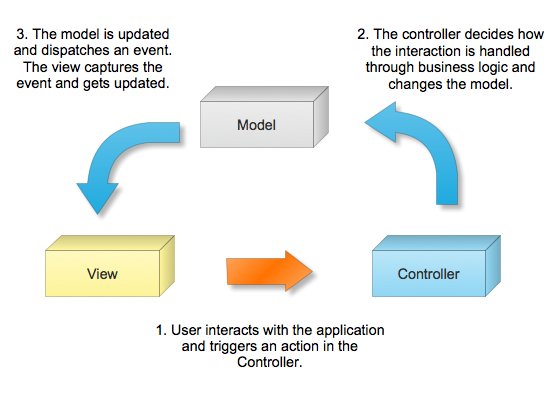
\includegraphics[width=\linewidth]
{pictures/MVC.png}
  \caption{The MVC pattern}
  \label{fig:mvc}
\end{figure}

\section{Runtime Management}\label{runtimeMng}





% Description of the management of threads and log procedures




\section{User interface}\label{interface}

We chose the Swing framework to develop the Pluto User Interface, already described in section \ref{plutoMainApp}.
We made this choice since Swing is well known to us.
Indeed we used it for the development of many academic projects, where we noticed that it allows to build graphical interface in a very fast and easy way and to add a great variety of components.
\\

Swing library is an official Java GUI toolkit released by Sun Microsystems. It is used to create Graphical user interfaces with Java.
The main characteristics of the Swing toolkit are:
\begin{itemize}
\item platform independent
\item customizable
\item extensible
\item configurable
\item lightweight
\end{itemize}

Swing is an advanced GUI toolkit. It has a rich set of widgets:
from basic widgets like buttons, labels, scrollbars to advanced like trees and tables. 
Swing itself is written in Java and is part of JFC, Java Foundation Classes: it is a collection of packages for creating full featured desktop applications.

There are basically two types of widget toolkits: \textit{Lightweight} and \textit{Heavyweight}.
A heavyweight toolkit uses OS's API to draw the widgets. For example Borland's VCL is a heavyweight toolkit since it depends on WIN32 API, the built in Windows application programming interface.
As already said, Swing is a lightweight toolkit since it paints its own widgets.

\section{The crazyflie nano-quadcopter}\label{crazyflie}

For the concrete actuation of the sensing tasks required by each application, we chose the Crazyflie Nano-Quadcopter, shown in figure \ref{fig:crazyflie}.


\begin{figure}[H]
\centering
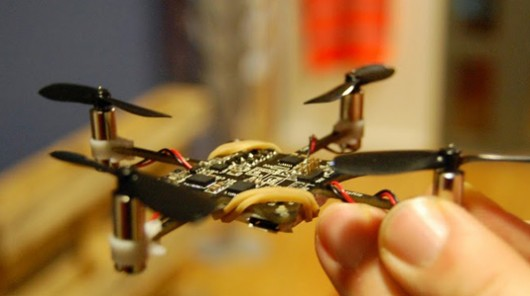
\includegraphics[width=\linewidth]
{pictures/crazyflie.jpg}
  \caption{The Crazyflie Nano-Quadcopter}
  \label{fig:crazyflie}
\end{figure}

The Crazyflie is a tiny quadcopter often referred to as a nano-quad, built using the PCB itself as the frame,developed solely by open source tools. The Crazyflie specs are the following:


\begin{itemize}
\item {Small and lightweight, around 19g and about 90mm motor to motor
}
\item {Flight time up to 7 minutes with standard 170mAh Li-Po battery
}
\item {Standard micro-USB connector for charging which takes 20min for the stock 170mAh Li-Po battery
}
\item {On-board low-energy radio@1mW based on the nRF24L01+ chip. Up to 80m range (environment dependent) when using the Crazyradio USB dongle}
\item{Radio bootloader which enables wireless update of the firmware
}
\item{Powerful 32 bit MCU: STM32F103CB @ 72 MHz (128kb flash, 20kb RAM)
}
\item{3-axis high-performance MEMs gyros with 3-axis accelerometer: Invensense MPU-6050
}
\item{Available footprints to manually solder magnetometer HMC5883L/HMC5983 or/and barometer MS5611
}
\item{4-layer low noise PCB design with separate voltage regulators for digital and analog supply
}
\end{itemize}

To concretely control the Crazyflie, there is a Python library which gives high level functions and hides the details.
We used a particular API to send the control command: 
\\

\begin{lstlisting}
	send_setpoint(roll, pitch, yaw, thrust)
\end{lstlisting}

The arguments roll/pitch/yaw/trust is the new set-points that should be sent to the copter.
For example, to send a new control set-point:
\\

\begin{lstlisting}
	 roll    = 0.0
    pitch   = 0.0
    yawrate = 0
    thrust  = 0
    crazyflie.commander.send_setpoint(roll, pitch, yawrate, thrust)
\end{lstlisting}

Changing the \textit{roll} and \textit{pitch} will make the quadcopter tilt to the sides and thus change the direction that it's moving in.
Changing the \textit{yaw} will make the quadcopter spin.
The thrust is used to control the altitude of the quadcopter.

By dynamically adjusting these four parameters we can make the Crazyflies move to the locations specified by the user through the Pluto User Interface.


